\section{Conception}

Avant la conception du projet il est nécessaire la prise en main du logiciel VLAB et l'utilisation des toolbox disponibles comme le toolbox\footnote{Un toolbox de VLAB est un compilation des librairies qui ajoutent des modeles de simulation pour VLAB, par exemple, le toolbox Ethernet nous donne des noeuds Ethernet, ports et la class de trame Ethernet pour l'envoie d'information.} CAN, Ethernet, LIN et aurix. J'ai d'abord instal\'e l'environement du travail avec les identifiants pour acceder \`a la reseaux interne de la soci\'et\'e. Deuxièmement, j'ai telecharge les dossiers du travail depuis les servers d'Australie. Apr\`es, j'ai compil\'e du logiciel simple pour tester le microcontr\^oleur (désormais appel\'e \textit{aurix}). Finalement, j'ai mod\'elis\'e quelques composants génériques pour tester des autres fonctionalit\'es du VLAB comme les connections des bancs de test, l'envoie de donn\'ees a travers des différents réseaux et la réception et utilisation de donn\'ees. Le développement de ce projet a \'et\'e divis\'e en 3 parties en fonction de l'évolution du même.

\begin{itemize}
    \item - Premier demo technique qui sers a faire la prise en main d'AUTOSAR, VLAB et l'environnement en général.
    \item - Developpement de l'aurix \textit{TC37xEXT}, pas support\'e jusqu'\`a moment du démarrage du stage.
    \item - Virtualisation du Gateway
\end{itemize}

\subsection{Premier demo technique}

Le premier exemple est fait pour tester le logiciel avec une configuration super simple. Il consiste a envoyer une trame CAN et le SWC la reenvoie vers le CANID source. Pour cet exemple une ECU générique a \'et\'e modélisé pour recevoir des trames CAN et LIN. Sur la figure \ref{fig:first-demo-diagram} se montre un diagrame de block des communications. 

Le structure de communications d'AUTOSAR de la figure \ref{fig:autosar-com-stack} nous montre que le chemin parcouru par les donn\'ees arrivant \'a l'aurix. Le chemin des donn\'ees de cette premier demo est le suivant \textit{Microcontroler}$ ->$ \textit{CAN\_Driver} $->$ \textit{CAN\_IF}\footnote{IF dans la notation AUTOSAR veut dire Interface} $->$ \textit{PDUR}\footnote{PDU est le nom des donn\'ees dans cette couche d'abstraction selon le mod\`ele OSI.}\footnote{PUDR est le router des PDUs. C'est ce module qui prends le décision o\`u envoyer les donn\'ees re\c cues}. C'est ici dans le PDUR qu'on trouve un probl\`eme parce que la trame re\c cue n'est pas activ\'e au début du programme.

\begin{figure}[!htb]
 \centering
 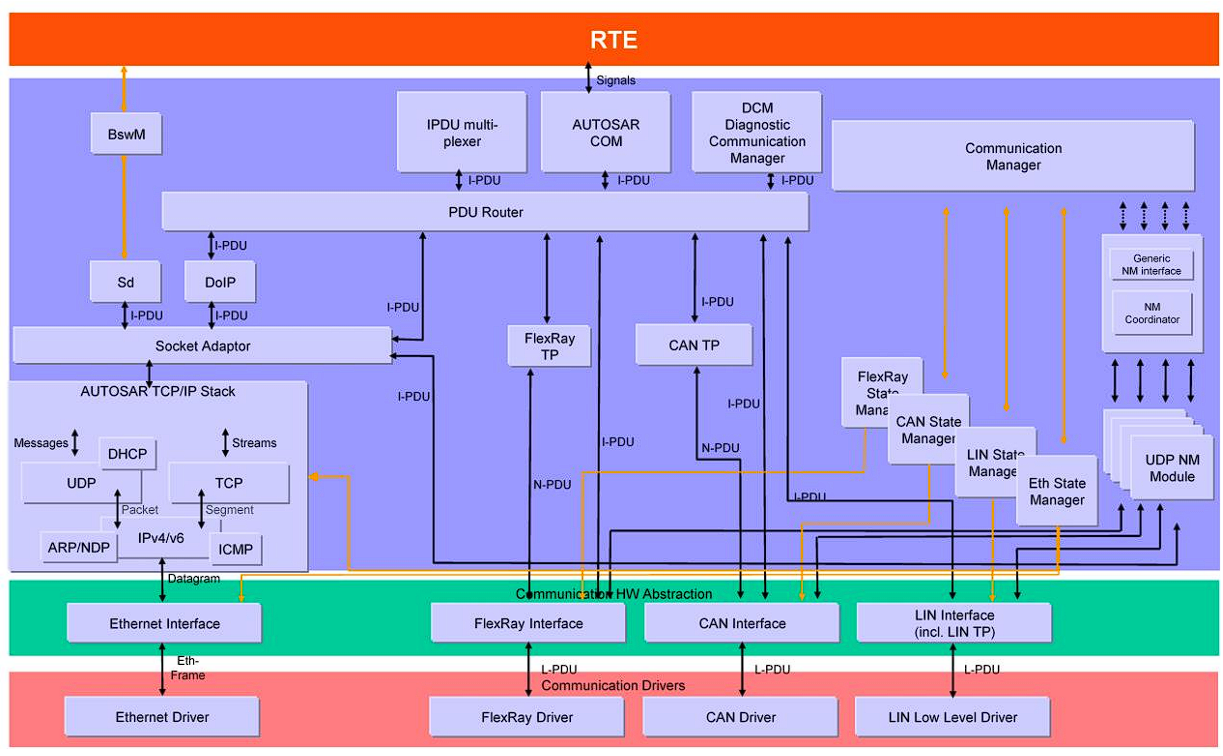
\includegraphics[width=\textwidth]{img/autosar_com_stack.png}
 \caption{Autosar Communication Stack}
 \label{fig:autosar-com-stack}
\end{figure}

Cette première demo a \'et\'e con\c cue pour \^etre test\'e avec le logiciel \textbf{CANoe} dont nous ne possédions pas la licence et le SWC n'a pas march\'e comme attendu. Les possibles explications sont las suivantes :

\begin{itemize}
    \item - Un protocole inconnu : Même si CANoe utilise le protocole CAN, il envoie peut \^etre d'autres trames d'identification avant le test.
    \item - Un SWC peu test\'e : Selon la documentation de ce test, ce SWC n'a pas \'et\'e teste au fond parce que son utilisation ne sera jamais implement\'e, c'est juste un test des logiciels.
\end{itemize}

Quand même, avec ce test j'ai acquis une connaissance basique du fonctionnement des logiciels AUTOSAR ce qui a rendu mon travaille future plus rapide et efficace. Un autre connaissance acquis dans ce partie c'était la partie de modélisation et le modèle de ECU déjà développe sera utilise plus tard.

\begin{figure}[!htb]
 \centering
 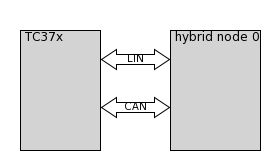
\includegraphics[]{img/first_demo_testbench.png}
 \caption{Premier demo}
 \label{fig:first-demo-diagram}
\end{figure}

\subsection{TC37xEXT}

Cette version de l'aurix ajoutait quelques modules de plus, les plus concernant pour ce projet c'etaient une interface CAN (MCMCAN\footnote{C'est le nom de l'interface CAN dans la famille de microcontroleurs \textit{aurix}}) et Gigabit Ethernet (GETH) de plus. Les autres differences seront trouv\'ees dans la table \ref{tab:tc37x_delta}. Le modèle du \textit{TC37x}\cite{aurix.tc37x} a \'et\'e pris comme la base et les interfaces et modules ont \'et\'e ajout\'es selon les adresses de base sur les buses correspondants.


% Table generated by Excel2LaTeX from sheet 'Sheet1'
\begin{table}[htbp]
  \centering
    \begin{tabular}{|r||l|l|}
	\hline
	\multirow{2}{*}{Module} & \multicolumn{2}{c|}{Aurix}\\
	\cline{2-3}
	& TC37x & TC37xEXT \\
	\hline \hline
	    RAM & TRAM (cached, non-cached) & EMEM (cached, non-cached) \\
	    \hline
	    CAN interfaces & 2 & 3 \\
	    \hline
	    Camera Interface & not present & CIF \\
	    \hline
	    Gigabit Ethernet Interface & 1 & 2 \\
	    \hline
	    SD interface & not present & present \\
	    \hline
	    eMMC interface & not present & present \\
	    \hline
	\hline
    \end{tabular}
  \caption{TC37x Vs TC37xEXT}
  \label{tab:tc37x_delta}
\end{table}


Pour ce type de modélisation les information sont fournies dans un fichier python qui fait l'assemblage de toutes les modèles de chaque module ou interface. Pour finaliser, il faut compiler et faire le test de chaque module ajout\'e.

Les testes doivent se faire en logiciel, il faut compiler un fichier \textit{.elf} et le monter sur la plateforme virtuelle cr\'e\'ee et lancer un script de test qui vérifie si tout se passe bien. Dans le cas precis du \textit{TC37xEXT},  nous avons test\'e l'accès aux registres de mémoire ajout\'e et des interfaces MCMCAN et GETH.

\subsection{Gateway Demo}

Les connections internes du gateway sont montr\'es dans la figure \ref{fig:devices-diagram}. \`A partir de cette configuration le testbench assembl\'e se montre dans la figure \ref{fig:connections-diagram}. %Dans ce point nous nous sommes rendu compte que le aurix utilis\'e n'etait pas celui de la application, ce gateway utilis\'e la version extended \cite{aurix.tc37e} de cet aurix donc j'ai du le developper.

\begin{figure}[!htb]
 \centering
 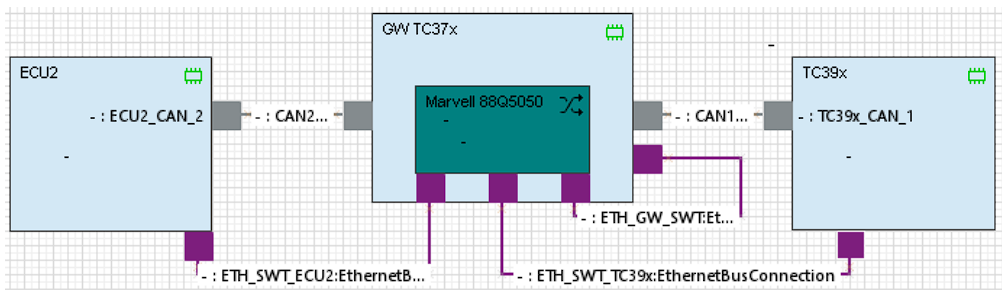
\includegraphics[width=\textwidth]{img/GWDemoConnections.PNG}
 \caption{Gateway Demo Devices}
 \label{fig:devices-diagram}
\end{figure}

\begin{figure}[!htb]
 \centering
 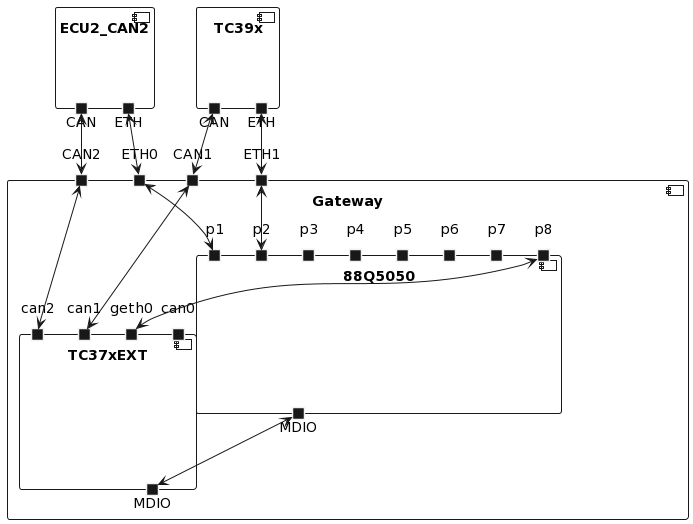
\includegraphics[width=\textwidth]{img/GWConnectionsDiagram.png}
 \caption{Gateway Connections Diagram}
 \label{fig:connections-diagram}
\end{figure}

\begin{figure}[!htb]
 \centering
 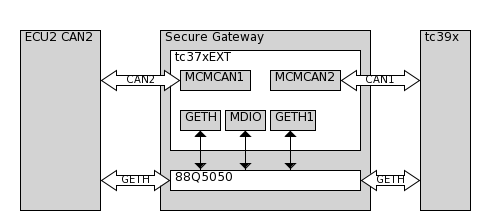
\includegraphics[width=\textwidth]{img/gateway_block_diagram.png}
 \caption{Gateway Block diagram}
 \label{fig:block diagram}
\end{figure}

\subsubsection{Switch Marvell 88Q5050}

Avant de demarrer les SWC le logiciel de la gateway verifie si toutes les composants et buses de donn\'ees sont presents. Un des composants present dans la carte est le Switch ethernet Marvell 88Q5050. C'est un switch securis\'e optimis\'e pour \^etre utilis\'e dans l'industrie automobile. Il est connect\'e aux ECUs externes via ports Ethernet et avec l'aurix a travers d'un port ethernet et un bus MDIO. Ce bus MDIO est utilis\'e pour accéder aux registres du switch a travers de l'aurix. De cette façon nous pouvons gérer le fonctionnement interne du switch avec l'aurix.

Ce modele a \'et\'e developp\'e en C++ et SystemC \`a l'aide du datasheet du fournisseur. Pour cette modèle j'ai suivi la procédure interne de modélisation des composants en ajoutant la quantit\'e  de buses, registres, ports et fonctionalit\'es de chaque élément. 

\subsubsection{Transceivers Marvell}

Ces transceivers connectent la couche PHY avec le switch. Avant le démarrage du logiciel le systeme de exploitation verifie son statut pour initialiser les ports.

Au moment de la rédaction de ce rapport, nous ne possédions pas les datasheet de ces transceivers.